\documentclass[a4paper]{article}
\usepackage[margin=3cm]{geometry}
\usepackage[utf8]{inputenc}
\usepackage{cmbright}
\usepackage[hidelinks]{hyperref}
\usepackage{booktabs}
\usepackage[ngerman]{babel}
\usepackage{parskip}
\usepackage{graphicx}
\usepackage{minted}
\usepackage{pdflscape}
\usepackage{array}
\usepackage{tabulary}
\usepackage{multicol}
\usepackage{pgfgantt}
\usepackage{pgf-umlcd}
\usepackage{enumitem}

% Page breaks between sections
\let\oldsection\section
\renewcommand\section{\clearpage\oldsection}

% JIRA/Confluence shortcuts
\def\jiraurl{https://jira.keltec.ch/jira}
\def\confluenceurl{https://jira.keltec.ch/wiki}
\newcommand{\jiraissue}[1]{\href{\jiraurl/projects/EPJ/issues/EPJ-#1}{EPJ-#1}}
\newcommand{\fulljiraissue}[1]{EPJ-#1 (\url{\jiraurl/projects/EPJ/issues/EPJ-#1})}

% Tools
\newcommand{\tool}[2]{\emph{#1\footnote{\url{#2}}}}

\begin{document}
	\title{
		Projekt: kitovu \\
		\Large{Software-Architektur} \\[3em]
		
\includegraphics[width=20em]{../../img/logo/kitovu.jpg}
	}
	\author{
		Florian Bruhin \\ \url{florian.bruhin@hsr.ch} \and
		Méline Sieber \\ \url{meline.sieber@hsr.ch} \and
		Nicolas Ganz \\ \url{nicolas.ganz@hsr.ch} 
		}
	\date{\today}
	
	\maketitle

\section*{Änderungsgeschichte}

\begin{tabulary}{\linewidth}{llLl}
	\toprule
	Datum & Version & Änderung & AutorIn \\
	\midrule
	28.03.2018 & 1.0 & Dokument erstellt, Grundgerüst von Template übernommen & Méline Sieber \\
	02.05.2018 & 2.0 & Abgabe Architektur-Review & alle \\

	\bottomrule
\end{tabulary}
\pagebreak

\section{Einführung}
Dieses Dokument legt dar, wie die Software-Architektur von \emph{kitovu} aufgebaut ist. Ein Abschnitt beschreibt die grafische Oberfläche, die wir zusätzlich zum Kommandozeilen-Client implementiert haben. Auch gehen wir auf die wichtigsten Abläufe des Clients ein. Im Kapitel zur logischen Architektur erläutern wir anhand von Grafiken die logischen Schichten von \emph{kitovu} und deren Zusammenhänge. Zudem klärt das Architekturdokument die grössten Risiken des Projekts, namentlich die Einbindung der beiden externen, als optional definierten Plattformen (Studentenportal, Moodle). Weiter erläutern wir auch die Herausforderung, die grafische Benutzeroberfläche mit dem Kommandozeilen-Client zu verbinden (Prozesse und Threads). Ein weiterer Punkt ist die Datenspeicherung, insbesondere der Aufbau der Konfigurationsdatei und des FileCache. Als letztes gehen wir noch auf die Skalierbarkeit ein, also, ob \emph{kitovu} auch für mehr Benutzerinnen und bei grösserem Synchronisationsaufwand zu gebrauchen ist.

Es bleibt eine Anmerkung: Viele Punkte der ``End of Elaboration'' definiert schon der sehr ausführliche Projektplan. Um dieses Dokument möglichst schlank zu halten, werden deshalb gewisse Punkte aussen vor gelassen, insbesondere die Ausführungen zur Grösse und Leistung von \emph{kitovu}. Für diesen Punkt sei auf den Projektplan verwiesen.

\subsection{Gültigkeitsbereich}
Die vorliegende Architekturbeschreibung ist für das Engineering-Projekt im Frühlingssemester 2018 gültig. Falls dem Projekt grössere Veränderungen widerfahren, wird das Dokument dementsprechend angepasst. Umfassende Änderungen werden am Anfang des Dokuments protokolliert.

\subsection{Referenzen}
Die Anforderungsspezifikation ist eng mit der Domainanalyse und anderen Dokumenten verbunden. Die folgende Tabelle listet die wichtigsten Referenzen auf.

\begin{tabulary}{\linewidth}{Ll}
	Confluence & \url{\confluenceurl} \\
	Draw.io & \url{https://www.draw.io/} \\
	Github-Repository von \emph{kitovu} & \url{https://github.com/kitovu-bot/kitovu} \\
	JIRA	& \url{\jiraurl} \\
	Moodle & \url{https://moodle.hsr.ch} \\
	Moodle Desktop & \url{https://download.moodle.org/desktop/} \\
	OpenHSR Connect & \url{https://github.com/openhsr/connect} \\
	Studentenportal & \url{https://studentenportal.ch/} \\
	Switch AAI \newline (Authentication and Authorization Infrastructure)& \url{https://www.switch.ch/aai/} \\
\end{tabulary}

Beim Logo auf der Titelseite handelt es sich um eine stark überarbeitete Version eines GIFs (\url{https://www.animateit.net/details.php?image_id=8990}). Urheber und Copyright sind nicht auffindbar.

\pagebreak

\section{Systemübersicht}

Das folgende Kontextprogramm verdeutlicht, wie die Schnittstellen von \emph{kitovu} aussehen. Auf der einen Seite  sind die Nutzerinnen und Nutzer, die je nach Informatikkenntnissen mit der grafischen Oberfläche oder mit dem Kommandozeilenprogramm interagieren. Auf der andere Seite sind die Plattformen, die \emph{kitovu} einbindet: Der Skripteserver sowie die Moodle-Plattform, die jedoch eine Authentifikation via Switch AAI verlangt. Weshalb das Studentenportal für dieses Projekt nicht implementiert werden kann, erklärt der nächste Abschnitt. \\

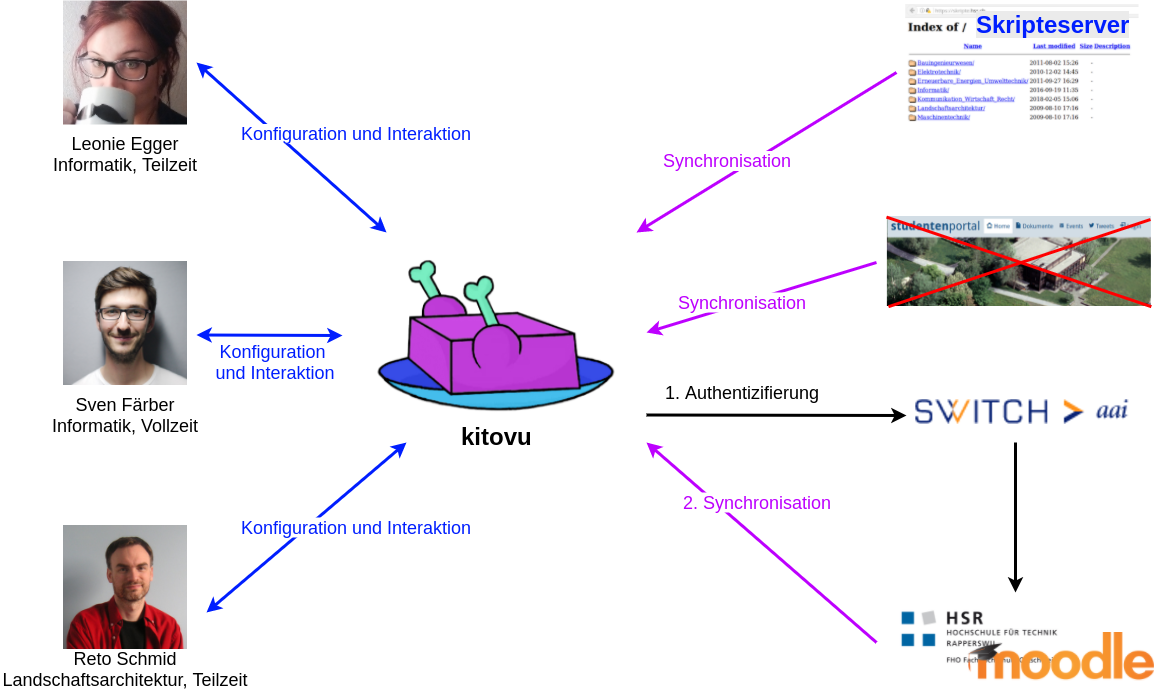
\includegraphics[width=40em]{./img/kontextdiagramm.png} \\

Die obigen drei Personas -- Leonie Egger, Sven Färber und Reto Schmid -- beschreibt die Anforderungsspezifikation ausführlich.

\section{Grafische Oberfläche}

% FIXME Als sub-section von Prozesse/Threads?

Als erste Iteration einer grafischen Oberfläche haben wir eine einfache GUI
entwickelt, welche \emph{kitovu} als Subprozess ausführt:

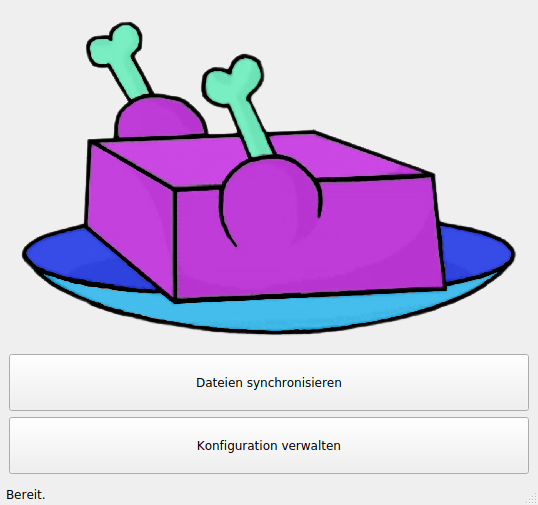
\includegraphics[width=0.5\linewidth]{./img/gui/gui1.png} \hspace{1em}
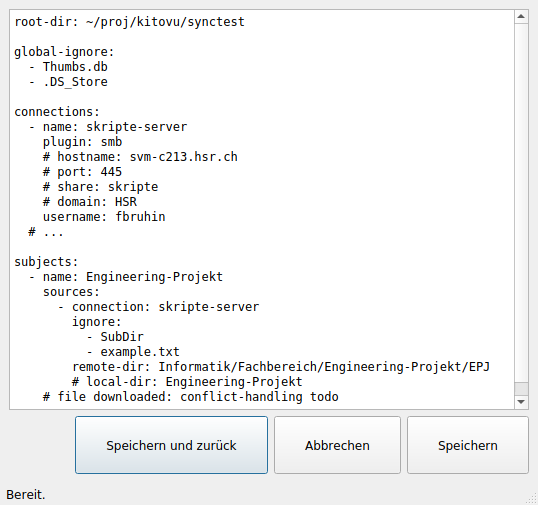
\includegraphics[width=0.5\linewidth]{./img/gui/gui2.png} \\[1em]
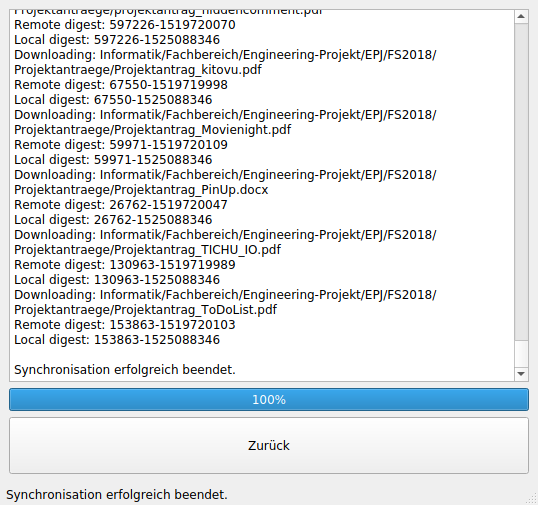
\includegraphics[width=0.5\linewidth]{./img/gui/gui3.png}

\section{Architektonische Ziele und Einschränkungen}

Der Projektplan erläuterte bereits die beiden grössten Risiken: Die Einbindung des Studentenportals und von Moodle, so dass sich von beiden Plattformen auch Dokumente synchronisieren lassen.

Zum Ende der Elaborationsphase zeigt sich, dass diese frühzeitige Einschränkung des Projekts sinnvoll war: Die Abklärung mit dem OpenHSR-Verein und den Betreibern des Studentenportals ergab, dass wir darauf verzichten müssen, das Portal einzubinden. Es fehlt an einer API, mit der wir Files synchronisieren können -- wir müssten dies von Hand hinzufügen, was jenseits des Projektumfangs liegt. Zudem sind viele Komponente des Studentenportals veraltet und sollten dringend aktualisiert werden. Ein möglicher Sprint sollte dem Abhilfe schaffen. Doch diesen organisiert die Fachschaft oder der OpenHSR-Verein und ist somit ausserhalb unseres Projekts. Das Studentenportal wird somit kein Teil von \emph{kitovu}.

Das zweite Risiko, die Moodle-Einbindung, ist noch in weiterer Abklärung. Ein erster Erfolg konnte verzeichnet werden: Der Moodle-Desktop-Client\footnote{\url{https://download.moodle.org/desktop/}} bzw. die mobile Version davon stellt bei erfolgreichem Login einen Moodle-Token zur Verfügung. Dank dieses Tokens ist es uns gelungen, via \emph{kitovu} ein File herunterzuladen. Eine erste Anbindung ist uns also gelungen. Noch offen ist, wie und ob wir die direkte Authentifikation via Switch AAI in \emph{kitovu} implementieren können; wir sind jedoch zuversichtlich, dass uns das gelingt.

\subsection{Wichtige Abläufe}

Synchronisationsprozesse haben einen kritischen Punkt: Die Datenintegrität. Denn die Daten sollen immer den Zustand behalten oder annehmen, wie die Nutzerin es sich wünscht. Um das zu gewährleisten, haben wir die Funktionalität des \verb|FileCache| definiert -- er führt Buch über den Zustand der Dateien\footnote{Vgl. auch Kapitel 6.}. Nach längeren Diskussionen haben wir folgende mögliche Fälle identifiziert, die während des Synchronisationsprozesses auftreten können:

\begin{tabulary}{\linewidth}{lLLLLl}
	\toprule
		\bfseries Fall &
	    \bfseries Situation Remote &
	    \bfseries Situation Lokal &
	    \bfseries Situation &
	    \bfseries Vorgehen &
	    \bfseries Enum-Wert\\
	\midrule

1 & nichts vorhanden &	lokal A &	remote gelöscht &	Konfliktbehandlung & 	\verb|REMOTE_CHANGED|*\\ \hline
2 & nichts vorhanden &	lokal A$'$ &	remote gelöscht, lokal geändert&	Konfliktbehandlung &	\verb|BOTH_CHANGED|*\\ \hline
3 & remote A &	nichts &	neue Datei existiert &	download &	\verb|NEW|\\ \hline
4 & remote B (neue Folien) &	lokal A (keine Änderungen) &	Folien-Update vom Dozent &	download &	\verb|REMOTE_CHANGED|\\\hline
5 & remote A &	lokal A &	keine Änderungen &	nichts& 	\verb|NO_CHANGES|\\\hline
6 & remote A &	lokal A$'$ (lokal geändert) &	lokale Notizen, kein Folien-Update &	update FileCache &	\verb|LOCAL_CHANGED|\\\hline
7 & remote B (neue Folien) &	lokal A$'$ (lokal geändert) &	beides geändert &	Konfliktbehandlung &	\verb|BOTH_CHANGED|\\
\bottomrule

\end{tabulary}

Die mit Sternchen (*) bezeichneten Einträge sind Spezialfälle. 

Aus der Tabelle wird ersichtlich, dass der \verb|FileCache| primär protokolliert, ob es jemals lokale Änderungen gab (aus A wurde A$'$). Mit anderen Worten: Wir müssen A separat -- im \verb|FileCache| -- abspeichern, um später feststellen zu können, ob sich in der Zeit bis zum nächsten Synchronisationsprozess die Datei geändert hat. 

\pagebreak

Daraus entstehen drei Digests:

\begin{itemize}
	\item Remote, der direkt aus der Remote-Datei berechnet wird
	\item Lokal im FileCache
	\item Lokal auf der Festplatte, also der Digest, der direkt aus der Datei berechnet wird.
\end{itemize}

Der \verb|FileCache| wird jeweils geschrieben, wenn die Datei heruntergeladen wird, und enthält zwei Werte: Den Digest zum Synchronisationszeitpunkt sowie den lokalen Dateipfad samt Dateinamen.

% FIXME Werte aktualisieren
Die oben definierten Enum-Werte \verb|NEW|, \verb|REMOTE_CHANGED|, \verb|LOCAL_CHANGED|, \verb|BOTH_CHANGED|, \verb|NO_CHANGES| verwenden wir, um die Konfliktbehandlung zu implementieren. Diese ist nötig, sobald sich die Datei lokal geändert hat (A$'$).

In der derzeitigen Entwicklungsphase des Clients haben wir uns vorerst für die Konfliktbehandlung ``overwrite'' entschieden. Selbst wenn sich die Datei zwischen zwei Synchronisationsprozessen geändert hat, wird sie also erneut von der Remote-Datei überschrieben.

Es ist uns jedoch ein Anliegen, dass sich diese Konfliktbehandlung von der Nutzerin steuern lässt, also dass sie in der Konfiguration von \emph{kitovu} festlegen kann, wie sich bei einem Konflikt das Programm verhalten soll (\emph{overwrite}, \emph{ignore}, \emph{rename}, \emph{ask}).

\subsection{Nicht-funktionale Anforderungen}

Die nicht-funktionalen Anforderungen, welche die Anforderungsspezifikation ausführt, haben wir erfüllt. Hier folgen Ergänzungen zu diesen Anforderungen.

\begin{tabulary}{\linewidth}{lL}
  \toprule
  Metrik & Beschreibung \\
  \midrule
  1.1.1. & Der \verb|FileCache| gewährleistet, geänderte Dateien zu erkennen. \\
  1.3.1. & Die Passwörter werden mit \verb|keyring| in den lokalen, betriebssystemspezifischen Passwort-Manager gespeichert. \\
  2.1.2. & \verb|Jsonschema| validiert die Konfigurationen und gibt die Fehler verständlich aus. \\
  4.1.1. & In Bezug auf das Skripteserver-Plugin muss pro Ordner ein Request abgesetzt werden, um die Liste aller Dateien zu erhalten. Ein zusätzlicher Request pro Datei ist nötig, um den Remote-Digest zu berechnen -- nur so können Datei-Attribute für den Digest abgefragt werden. Pro Datei, welche sich geändert hat, wird ein weiterer Request abgesetzt um den Inhalt zu laden. \[ N_{Requests} = N_{Ordner} + N_{Dateien} + N_{ge"anderte Dateien} \] \\
  \bottomrule
\end{tabulary}

\section{Logische Architektur}

% <Beschreibung der logischen Struktur des Projekts. Pro Subsystem/Package ein einzelner Abschnitt und ein Übersichtsdiagramm über die einzelnen Subsysteme/Packages. Aufteilung in Subsysteme/Packages (zum Beispiel: 3-Layer-Architektur mit GUI, Problem Domain und Datenhaltung). >

% Weitere Punkte: Klassenstruktur, Schnittstellen, Wichtige interne Abläufe, Wichtige Abläufe

\subsection{Schichten}

Das folgende Diagramm veranschaulicht, wie der Code von \emph{kitovu} aufgebaut ist und wie die einzelnen Packages miteinander interagieren.

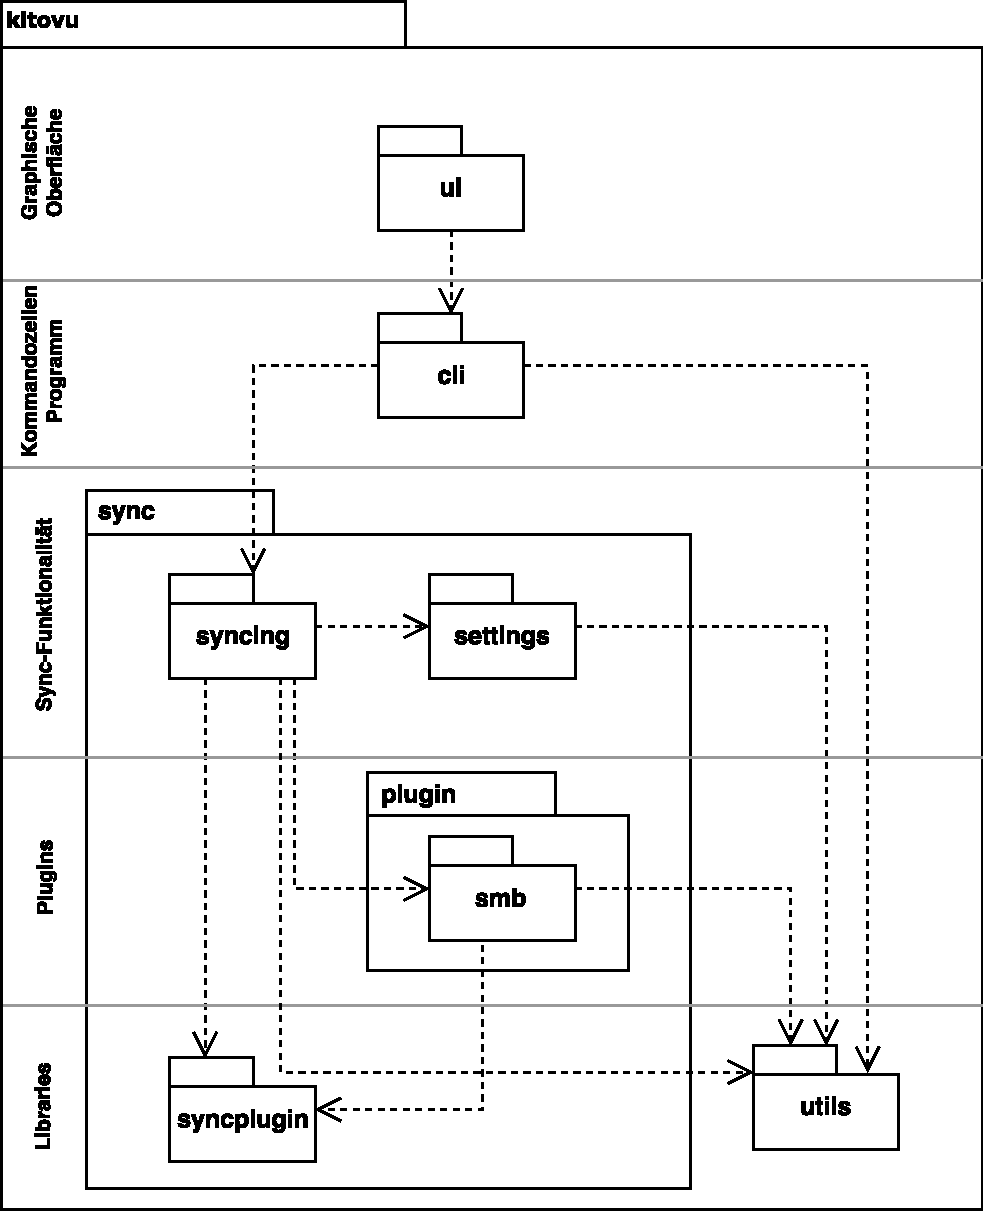
\includegraphics[width=40em]{./img/schichtendiagramm.pdf}

\newpage

\subsection{Sequenzdiagramm}

Das Sequenzdiagramm beschreibt, wie die Funktionen eines Plugins aufgerufen werden.
Dies sollte Plugin-Entwicklern helfen zu verstehen, wie die Synchronisation abläuft.

Die \verb|Settings| sind aufgeführt um zu zeigen, dass die Plugins in Abhängigkeit zu den \verb|Settings| geladen werden.

Ein grösserer Punkt ist der \verb|FileCache| -- dieser fehlt bewusst im Diagramm.
Dieser hat jedoch keinen Einfluss auf die Plugins, sondern es sind Auslagerungen der Funktionalitäten des \verb|syncing| Namespaces.
%FIXME verständlichkeit?

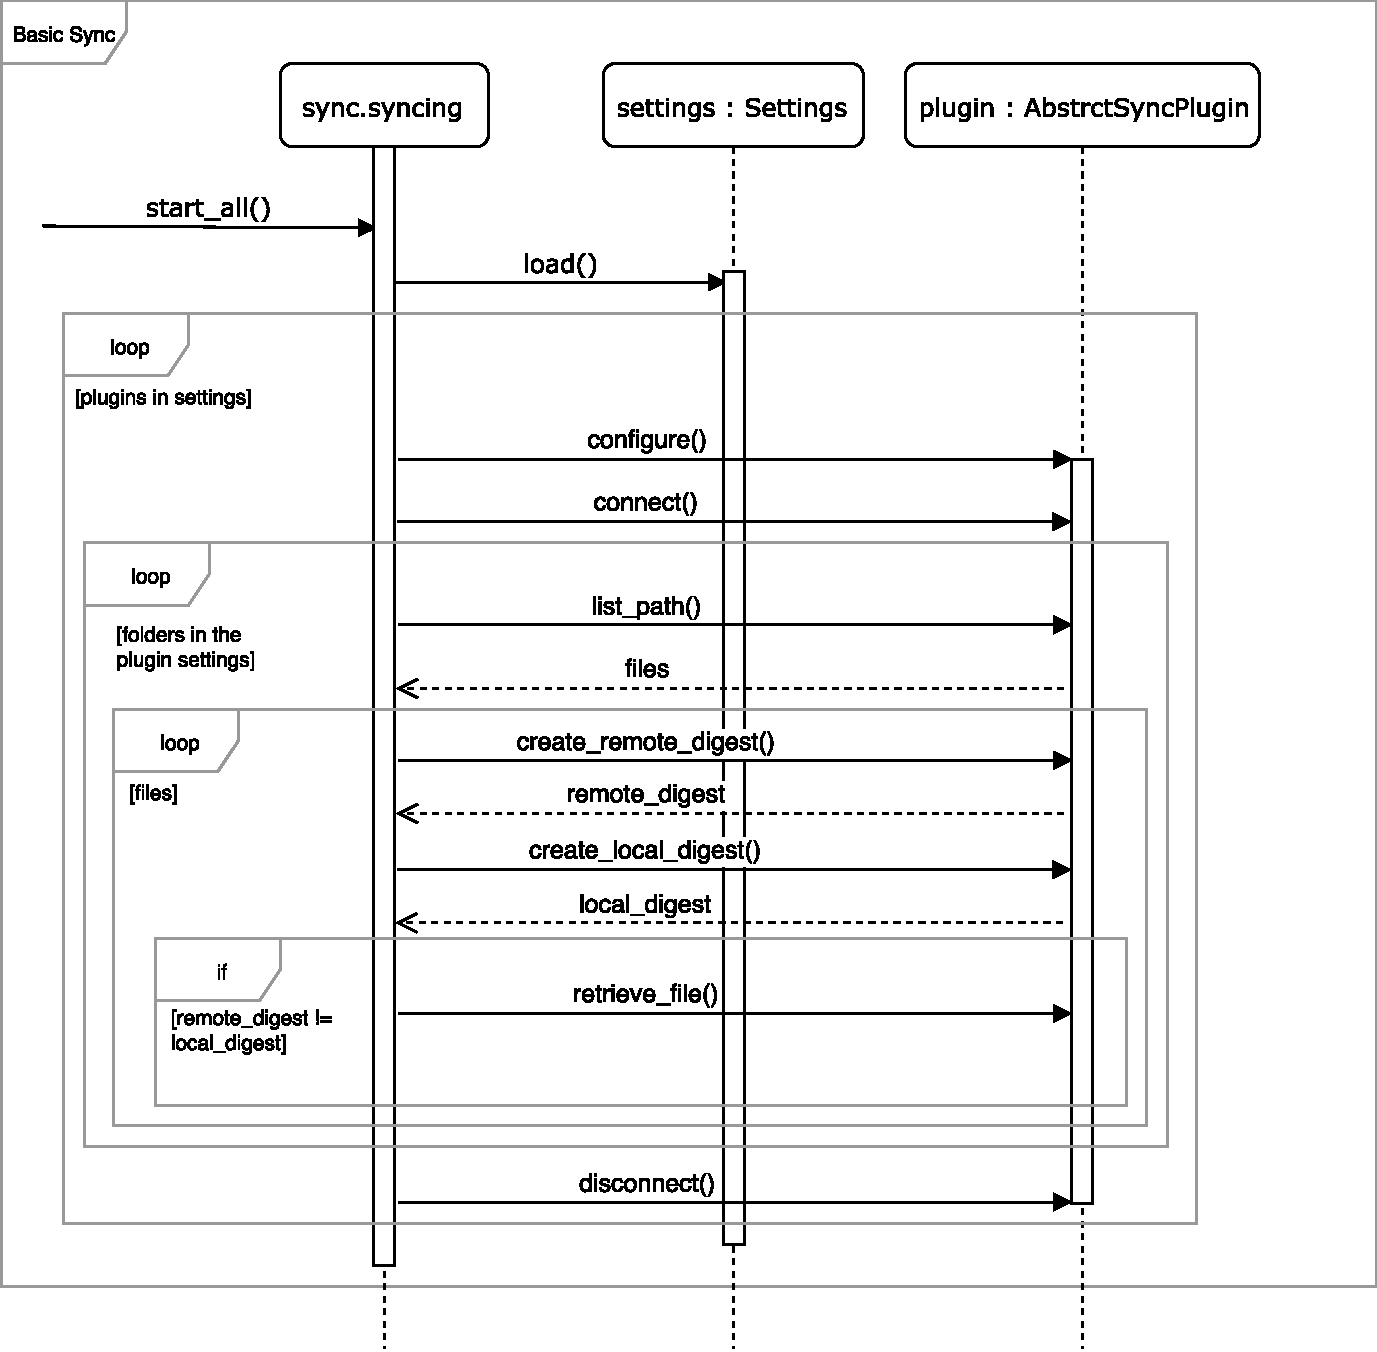
\includegraphics[width=40em]{./img/GrobesSequenzDiagramm.pdf}

\pagebreak
\subsection{Wichtigste Klassen}

Die Domainanalyse aus der Anforderungsspezifikation ist bis auf einige kleine
Änderungen weiterhin so gültig. Deshalb verzichten wir in diesem Dokument
darauf, ein erneutes Domainmodell aufzuführen. Nachfolgend sind die wichtigsten
Klassen im Projekt tabellarisch als grobe Kurzübersicht nochmals aufgeführt.

\begin{tabulary}{\linewidth}{llLl}
	\toprule
	Klasse & Package & Funktion \\
	\midrule
  \verb|StartScreen| & \verb|gui| & Die verschiedenen Ansichten der GUI. \\
  \verb|SyncScreen| & & \\
  \verb|ConfScreen| & & \\
  \hline
  \verb|AbstractSyncPlugin| & \verb|sync| & Abstrakte Basisklasse für Synchronisations-Plugins. \\
  \verb|SmbPlugin| & \verb|sync| & Implentation des Plugins für die SMB-Kommunikation (Skripteserver). \\
  \verb|MoodlePlugin| & \verb|sync| & Implentation des Plugins für die Moodle-Kommunikation. \\
  \verb|DummyPlugin| & \verb|tests.helpers| & Implementation eines Plugins mit fiktiven Daten für Tests. \\
  \hline
  \verb|Settings| & \verb|sync| & Code für das Einlesen und Abfragen der Konfiguration. \\
  \verb|ConnectionSettings| & \verb|sync| & Konfiguration für eine einzelne Verbindung. \\
  \hline
  \verb|FileCache| & \verb|sync| & Zuständig dafür, Änderungen in Dateien (lokal/remote) nachzuverfolgen. \\
  \hline
  \verb|AbstractReporter| & \verb|utils| & Abstrakte Basisklasse für die Meldung von Warnungen an den Core-Teil aus einem Plugin. \\
  \verb|CliReporter| & \verb|utils| & Fehler-Reporting für den Kommandozeilen-Client. \\
	\bottomrule
\end{tabulary}

\pagebreak

\subsection{Plugin-Architektur}

Wir wollten von Beginn weg \emph{kitovu} so entwerfen, dass der Client sich leicht ausbauen lässt, da ja an der HSR die Unterrichtsmaterialien von verschiedenen Quellen synchronisiert werden. Eine weitere Überlegung war, dass künftige Studierende selber \emph{kitovu} erweitern können, so dass sie neue oder andere Plattformen selbständig einbinden können. Dies veranschaulicht bereits die Persona der Leonie Egger. 

Deswegen entschieden wir, \emph{kitovu} mittels einer Plugin-Architektur aufzubauen, so dass neue Plattformen einfach als neue Plugins geschrieben werden können. Via des ``Template Method''-Pattern werden diese Plugins in \emph{kitovu} eingehängt. So ist es theoretisch möglich, eine Vielzahl von externen Plattformen in \emph{kitovu} zu integrieren, ohne dass der gesamte Code umgeschrieben werden muss.

Nach einer ersten Evaluation erwies sich die ursprüngliche Plugin-Architektur \verb|pluggy| als unbrauchbar. Wir haben \verb|pluggy| verworfen, da es eine andere Architektur für Plugins
voraussetzt: Es erwartet eine Architektur, bei der der
Core-Teil eine Methode aufruft, und diese Methode dann in allen verfügbaren
Plugins aufgerufen wird (\emph{Hooks}, ähnlich des ``Observer''-Patterns). Wir benötigen hingegen eine Architektur, bei der wir das Plugin anhand der Konfiguration aussuchen können -- danach interagieren wir nur noch mit diesem einen Plugin.

Wir entschieden uns deshalb für die \verb|stevedore|-Bibliothek.\footnote{\url{https://docs.openstack.org/stevedore/latest/}} \verb|Stevedore| ist mächtiger als \verb|pluggy|, da sie sowohl das \emph{Hook}-Pattern unterstützt als auch das ``Template''-Pattern, das wir benötigen. \verb|Stevedore| nennt das für uns interessante und in \emph{kitovu} verwendete Pattern ein ``Driver''-Pattern: \\

\begin{center}
	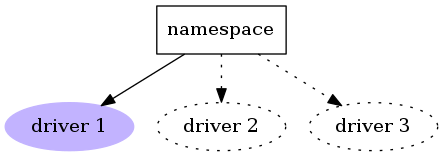
\includegraphics[height=8em]{img/stevedore_driver.png}
\end{center}

Als Vergleich das ebenfalls mögliche ``Hook''-Pattern von \verb|stevedore|, welches der
Funktionsweise von \verb|pluggy| ähnelt:

\begin{center}
	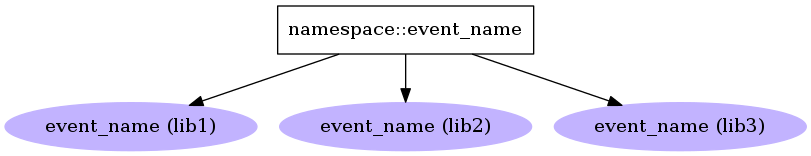
\includegraphics[height=8em]{img/stevedore_hooks.png}
\end{center}

Die obigen Grafiken stammen aus der \verb|stevedore|-Dokumentation.

\section{Fehlerbehandlung}
Wir haben uns dafür entschieden, die Fehlerbehandlung grösstenteils basierend
auf Exceptions zu implementieren -- ein Vorgehen, welches in der Python-Welt
vermutlich weiter verbreitet ist als in der Java-Welt. Die genaueren Gründe für
dieses Vorgehen werden nachfolgend dargelegt.

Sofern keine entsprechenden Bugs in \emph{kitovu} vorhanden sind, schätzen wir die
Chancen für einen Übertragungsfehler sehr gering ein. Wir können bereits auf robusten Protokollen aufbauen
(TCP, SMB, HTTP) und erwarten deswegen eine zuverlässige Datenübertragung. Dieses Problem ist also von uns abstrahiert.

In anderen Sprachen werden oft ``Error-Objekte'' selbst konstruiert. Werden
zusätzliche Informationen benötigt -- beispielsweise welche Funktion genau fehlschlug --, so muss dies mühsam von Hand übergeben werden.

In Python werden oft Exceptions als solche Error-Objekte benutzt. Es handelt
sich bei Exceptions in Python um \emph{first-class
  objects}\footnote{\url{https://en.wikipedia.org/wiki/First-class_object}}, sie
können also auch problemlos in einer Liste gespeichert und weitergegeben werden.
Ausserdem sind Exceptions sehr leichtgewichtige Konstrukte, im Gegensatz zu z.B.
Java\footnote{\url{https://shipilev.net/blog/2014/exceptional-performance/}}.

Wichtig für die Architektur ist die Entscheidung, bei welchen Problemen wir
welche Operation abbrechen wollen:

\begin{itemize}
  \item Jegliche unbehandelte Exception (Bug) $\rightarrow$ ganzes Programm bricht ab
  \item Verbindung zum Server bricht im Plugin ab $\rightarrow$ nur das
    entsprechende Plugin wird ignoriert. Error-Handling-Code soll möglichst
    simpel sein; neuer Verbindungsaufbau nach Verbindungsabbruch macht
    vermutlich mehr Probleme, als es löst.
  \item Fehler beim Herunterladen einer Datei $\rightarrow$ Datei wird
    übersprungen, der Rest des Plugins läuft trotzdem weiter.
\end{itemize}

Gerade bei Verbindungsfehlern enthält die Exception, die die entsprechende
Library (PySMB, requests, etc.) wirft, schon nützliche Informationen. Deshalb
macht es Sinn, diese Exception beizubehalten und zu behandeln, damit diese
Informationen nicht verloren gehen, da sie z.B. auch für Debugging-Zwecke verwendet werden können.

\section{Prozesse und Threads}

% <Wenn mehrere Prozesse oder Threads eingesetzt werden wird hier beschrieben, wie diese ablaufen, miteinander funktionieren, Daten austauschen, sich synchronisieren, usw.>

Die grafische Implementation von \emph{kitovu} stellt uns vor die Herausforderung, wie die Bibliotheken zur Synchronisation in die GUI eingebunden werden, da diese nicht blockiert werden darf. Dazu gibt es mehrere Lösungsansätze:

\begin{enumerate}
	\item Zwei separate Prozesse: Die GUI läuft in einem separaten Prozess und kommuniziert mit dem Kommandozeilen-Prozesses, der die Synchronisation übernimmt.
	\item Zwei Threads: Die Bibliotheken zur Synchronisation laufen in einem separaten Thread im gleichen Prozess wie die GUI.
	\item Verwenden von asynchronen Bibliotheken (\verb|asyncio| oder \verb|twisted|), die im gleichen Thread wie die GUI die Synchronisation durchführen können, ohne die GUI zu blockieren.
\end{enumerate}

Für den Kommandozeilen-Client nehmen wir in Kauf, dass der Client blockiert wird, wenn er die Synchronisation durchführt.

Für den GUI-Protoyp wählen wir die erste Lösung oben in der Liste. Der grafische und textbasierte Client implementieren wir also als zwei separate OS-Prozesse. Für ein besseres GUI sollte dies jedoch via Threads oder einer Python-Bibliothek für asynchrone Programmierung erfolgen (dritte Variante oben). Hier folgen wir dem Projektplan und nehmen an, dass diese Implementation nicht mehr Teil des Engineering-Projekts sein wird.

\section{Datenspeicherung}

% <Beschreibung mit Diagramm der Datenspeicherung (Datenmodell, z.B. Datenbank)>
\subsection{Konfigurationsdatei}
Die Konfigurationsdatei soll so gestaltet sein, dass auch Studierende ausserhalb des Informatikstudienganges damit umgehen könnten. Die Verständlichkeit steht also im Vordergrund. So ist sie aufgebaut:

\begin{minted}{yaml}
root-dir: ~/Documents/HSR/semester_06

global-ignore:
  - Thumbs.db
  - .DS_Store

connections:
  - name: skripte-server
    plugin: smb
    # hostname: svm-c213.hsr.ch
    # port: 445
    # share: skripte
    # domain: HSR
    username: nganz
  # ...

subjects:
  - name: Engineering-Projekt
    sources:
      - connection: skripte-server
        ignore:
          - SubDir
          - example.txt
        remote-dir: Informatik/Fachbereich/Engineering-Projekt/EPJ
        # local-dir: Engineering-Projekt
\end{minted}

Wir haben uns für diese Struktur entschieden, da damit die Plugins sehr dynamisch konfiguriert werden können.

Der Abschnitt zu \verb|connections| konfiguriert einzelne Plugins.
Da diese einen spezifischen Namen haben, kann ein Plugin auch mehrmals verwendet werden.
Dies ist nützlich, wenn es in einer anderen Schule zum Beispiel mehrere SMB-Server hat.
Dann kann pro Server eine \verb|connection| gesetzt weren.

Die \verb|subjects| sind Gruppierungen nach besuchtem Fach.
Ein Fach hat so mehrere \verb|sources|, welche unterschiedliche \verb|connetions| verwenden können.
Dadurch kann für ein Fach z.B. die Synchronisation des Skripte-Servers als auch von Moodle eingerichtet werden.

Ein \verb|subject| bezeichnet also ein Unterrichtsmodul an der HSR -- aufgrund möglicher Begriffskonfusionen haben wir uns für den abstrakteren Begriff entschieden, statt Bezeichnungen wie \verb|location|, \verb|module| oder \verb|places|.

\pagebreak

\subsection{FileCache}

Zum Bereich der Datenspeicherung gehört ebenfalls der \verb|FileCache|, dess Funktionalität bereits das Kapitel ``Wichtige Abläufe'' genauer beschrieben hat. Er ist im Wesentlichen eine lokale Speicherung des \verb|remote_digest|, der zum Zeitpunkt des letzten Synchronisationsvorgangs erstellt wurde. Anhand des \verb|FileCache| kann so zu einem späteren Zeitpunkt verglichen werden, ob sich bis dahin die lokale Datei geändert hat.

Im Gegensatz zur Konfigurationsdatei, die als \verb|YAML|-Datei gespeichert wird, speichern wir den \verb|FileCache| als \verb|JSON|-Datei. Der Vorteil einer \verb|JSON|-Datei ist die reduzierte Dateigrösse sowie bessere Performance. Zudem ist diese Datei nicht dazu gedacht, von Personen gelesen zu werden, in Kontrast zur Konfigurationsdatei.

Ein Eintrag in der \verb|filecache.json| sieht nun folgendermassen aus:

\begin{minted}[breaklines]{json}
{"/home/legger/kitovu/EPJ/SoftwareArchitektur.docx": 
	{"plugin": "smb", 
	"digest": "36837-1525097547"}}
\end{minted}

Er wird je nach Betriebssystem an einem anderen Ort hinterlegt. 

Für Linux: \verb|~/.local/share/kitovu/filecache.json|,

für Windows: \verb|C:\Users\legger\AppData\Local\kitovu\filecache.json|.

Gemäss unseren Berechnungen zu den Dateimengen in der Anforderungsspezifikation erwarten wir, dass diese Datei am Ende des Semesters rund 7000 Einträge umfasst, mit 1000 Einträgen pro Modul. Wir schätzen dies als eine handhabbare Grösse für den \verb|FileCache| ein.

\section{Skalierbarkeit}

\subsection{Mehr externe Plattformen}

Für das Engineering Projekt haben wir \emph{kitovu} in minimal möglichem Umfang geplant: Die Synchronisation mit dem Skripteserver muss funktionieren. Alle weiteren externen Plattformen haben wir als optional definiert, auch aufgrund möglicher Risiken -- die sich im Fall des Studentenportals als berechtigt erwiesen haben. Von Anfang an planten wir jedoch die Erweiterbarkeit von \emph{kitovu}, wie wir bereits oben im Abschnitt zur Plugin-Architektur erläutert haben. 

Das ist nun problemlos möglich: Entgegen unseren kalkulierten Risiken ist eine Moodle-Anbindung möglich -- und lässt sich nun dank der Plugin-Architektur problemlos integrieren. \emph{Kitovu} skaliert also für mehr als eine Plattform.


\subsection{Mehr Nutzerinnen und Nutzer}

Vor und während der Projektarbeit haben wir festgestellt, dass \emph{kitovu} auf grossen Anklang stösst: Viele HSR-Studentinnen und -Studenten wünschen sich eine einfache Möglichkeit, ihre Unterrichtsmaterialien à jour zu halten. Wir hoffen deshalb und erwarten, dass der Client häufig und von vielen genutzt wird.

\emph{Kitovu} wird lokal bei den Nutzerinnen und Nutzern installiert, das Programm dürfte also problemlos skalieren, da mehr Nutzer keine grössere Last für den einzelnen Client bedeuten. Das einzige Problem wäre, dass die vielen Server-Anfragen von \emph{kitovu} den Skripteserver zum Erliegen bringen. Wir schätzen dieses Risiko jedoch als gering ein und erwarten von der Schulinfrastruktur, dass sie allfällige Spitzen von Netzwerkanfragen verarbeiten mag. Wir erwarten sogar, dass  \emph{kitovu} den Skripteserver \emph{weniger} belastet: Momentan laden viele Studierende alle Dateien oft neu herunter, während \emph{kitovu} nur geänderte Dateien herunterlädt.

\end{document}
